\chapter{Datasets}
This chapter contains dataset information

\subsection{Notation}
As already stated, we define a time series dataset used within as  $\{x_{t}^{(m)}\}$.  Each $x_{t}^{m}$ is an aggregate of the readings from sensor $m$ reading at time block $t$. 

Forecasts for a given model $k$ from the set of all models $K$ are represented by 
\begin{equation}
\bar{T}_{t + 1}^{k, m} = f(T_{t}, ..., T_{1}; \theta_{k}).
\end{equation}
\noindent
Thus the forecast of $T_{t + 1}$ is a function of all past data and some trained parameterization $\theta_{k}$ for that model. 

In this work we need to forecast more than one time step into the future.  Future forecasts are performed through iterative one step ahead forecasts.  Also for this work we forecast a model for each individual sensor and for convenience drop the $m$ from our forecasting notation.  An example of a forecast two time steps ahead of current time $t$ is given by 
\begin{equation}
\bar{T}_{t + 2}^{k} = f(\bar{T}_{t + 1}, T_{t}, ..., T_{1}; \theta_{k}).
\end{equation}
\noindent
Such a forecast is simply the forecast for one time step into the future but now with the forecasted value of $\bar{T}_{t + 1}$ used as the most recent datapoint to forecast $\bar{T}_{t + 2}$.  Forecasting in this nature allows for forecasts any number of time steps into the future. 

\subsection{Forecast measurements}
Discuss MAPE, MASE, RMSE, and our approach here

TODO: Perhaps remove this to another section
This could be represented by a hypothesis function $h(x, \delta)$.  We use mean absolute scale error (MASE) \cite{Hyndman2006} and root mean squared error (RMSE) as cost functions to compare with other previously implemented techniques.

\subsection{MERL Dataset} 

The Mitsubishi Electronic Research Labs dataset is derived from a collection of over 200 passive infrared sensors place densely throughout the 7th and 8th floor of a research office building.  The sensors are placed roughly two meters apart on the ceilings, creating a dense sensing area with little non-sensed space.  Readings are taken at the millisecond level, but due to the sensors' settling times the inter-detection time of motion is approximately 1.5 seconds.

The data was collected from March 2006 through March 2008 and there are roughly 53 million sensor readings.  This building is similar to most office buildings with a number of personal offices along with labs and conference rooms.  Employees have roughly set schedules and holidays are observed as normal. 

The counts of sensor activations have been aggregated every 10 minutes.  Because of the lack of significant motion in the night, we look only at activations that occur between 6:00am and 7:00pm daily.  A plot of the average activations of all Wednesdays for a single sensor along with a range of one standard deviation is given in Figure~\ref{fig:merlday}.  

Peak motion unsurprisingly occurs during the middle of the day corresponding to lunch time.  There is another small peak of motion near the start of the day corresponding to people entering.  Near the end of the day, instead of a peak there is a region corresponding to high variance.  This seems to imply that while people enter at roughly the same time, there is a significant variance on when people leave the building.


\subsection{Colorado School of Mines Dataset}

The Colorado School of Mines dataset is a collection of 50 passive infrared sensors mounted on the ceiling of the second floor of a class and office room building.  The density of the sensor placement depends on the location within the building.  Outside the auditorium in the lower right of Figure~\ref{fig:csmbbfloor} is a dense collection of sensors placed approximately every few meters.  Throughout the rest of the building the sensors are placed roughly every 5 meters.  Data was collected for one academic school year from 2008 to 2009 and there are more than 23 million sensor readings.  To acquire readings, the sensors were polled every second and recorded data if motion was detected.  

%\begin{figure}[h]
%\begin{center}
%	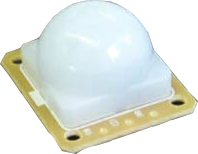
\includegraphics[width = .4\linewidth]{pir_sensor}
%	\caption{Passive infrared motion detector}
%\end{center}
%\end{figure}

%\begin{figure}[h]
%	\begin{center}
%		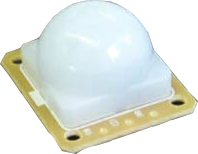
\includegraphics[width = .4\linewidth]{pir_sensor.png}
%		\caption{Passive infrared motion detector}
%	\label{fig:pirsensor}
%	\end{center}
%\end{figure}

%\begin{figure*}[t!]
%\centering
%\begin{subfigure}{.45\textwidth}
%  \centering
%  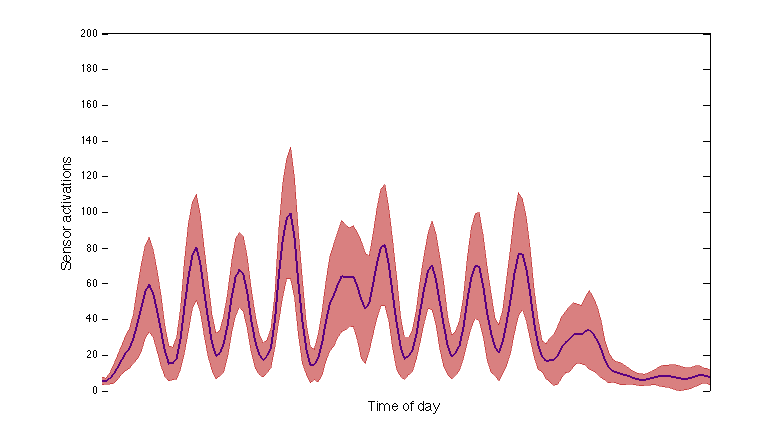
\includegraphics[width=1.0\linewidth]{brown_day.png}
%  \caption{CSM Brown Building average of all Wednesdays}
%  \label{fig:csmday}
%\end{subfigure}
%\begin{subfigure}{.45\textwidth}
%  \centering
%  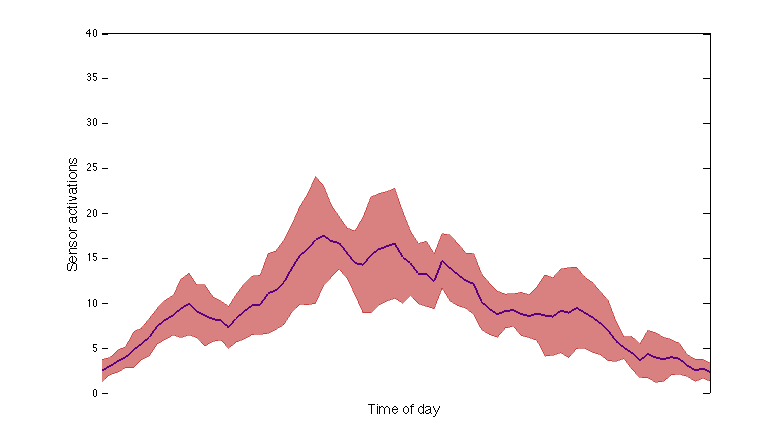
\includegraphics[width=1.0\linewidth]{merl_day.png}
%  \caption{MERL average of all Wednesdays}
%  \label{fig:merlday}
%\end{subfigure}
%\caption{Average sensor activations for a specific sensor on Wednesdays with one standard deviation range.}
%\label{fig:dayplot}
%\end{figure*}

This dataset is much different than the MERL dataset as classes typically provide activity on a rigid schedule during the day.  Also as students have exams and projects, late night motion is sporadic based on the time of year.  The counts of sensor activations have been aggregated over every 10 minutes.  Despite occasional late night motion during exam time, most nights have no significant motion.  For this reason we focus on data between 7:00am and 7:00pm daily.  A plot of the average activations of all Wednesdays for a single sensor along with a range of one standard deviation is given in Figure~\ref{fig:csmday}.  The defined peaks in the dataset correlate to class start and end times when most students will be in the hallways of the building.

\subsection{Denver traffic dataset}
Discuss the denver traffic dataset here.